% Created by tikzDevice version 0.6.2-92-0ad2792 on 2013-11-02 06:59:26
% !TEX encoding = UTF-8 Unicode
\documentclass[12pt, mainfont = Minion,     mainscale = 1.0, sansfont = Myriad,     sansscale = MatchLowercase, monofont = Consolas,   monoscale = MatchLowercase, mathfont = MinionMath, mathscale = 1.0]{mtikzfig}
\begin{document}

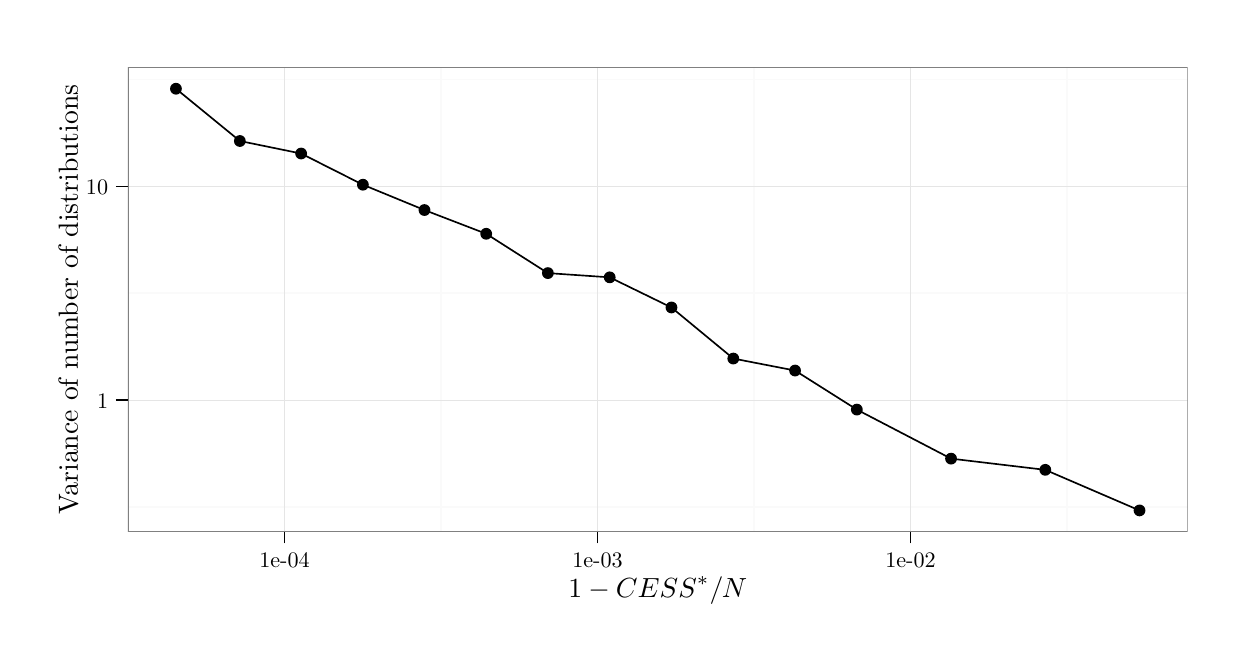
\begin{tikzpicture}[x=1pt,y=1pt]
\definecolor[named]{fillColor}{rgb}{1.00,1.00,1.00}
\path[use as bounding box,fill=fillColor,fill opacity=0.00] (0,0) rectangle (433.62,216.81);
\begin{scope}
\path[clip] (  0.00,  0.00) rectangle (433.62,216.81);
\definecolor[named]{drawColor}{rgb}{1.00,1.00,1.00}
\definecolor[named]{fillColor}{rgb}{1.00,1.00,1.00}

\path[draw=drawColor,line width= 0.6pt,line join=round,line cap=round,fill=fillColor] ( -0.00,  0.00) rectangle (433.62,216.81);
\end{scope}
\begin{scope}
\path[clip] ( 36.18, 34.74) rectangle (419.17,202.36);
\definecolor[named]{fillColor}{rgb}{1.00,1.00,1.00}

\path[fill=fillColor] ( 36.18, 34.74) rectangle (419.17,202.36);
\definecolor[named]{drawColor}{rgb}{0.98,0.98,0.98}

\path[draw=drawColor,line width= 0.6pt,line join=round] ( 36.18, 43.58) --
	(419.17, 43.58);

\path[draw=drawColor,line width= 0.6pt,line join=round] ( 36.18,120.83) --
	(419.17,120.83);

\path[draw=drawColor,line width= 0.6pt,line join=round] ( 36.18,198.08) --
	(419.17,198.08);

\path[draw=drawColor,line width= 0.6pt,line join=round] ( 36.26, 34.74) --
	( 36.26,202.36);

\path[draw=drawColor,line width= 0.6pt,line join=round] (149.36, 34.74) --
	(149.36,202.36);

\path[draw=drawColor,line width= 0.6pt,line join=round] (262.46, 34.74) --
	(262.46,202.36);

\path[draw=drawColor,line width= 0.6pt,line join=round] (375.56, 34.74) --
	(375.56,202.36);
\definecolor[named]{drawColor}{rgb}{0.90,0.90,0.90}

\path[draw=drawColor,line width= 0.2pt,line join=round] ( 36.18, 82.21) --
	(419.17, 82.21);

\path[draw=drawColor,line width= 0.2pt,line join=round] ( 36.18,159.46) --
	(419.17,159.46);

\path[draw=drawColor,line width= 0.2pt,line join=round] ( 92.81, 34.74) --
	( 92.81,202.36);

\path[draw=drawColor,line width= 0.2pt,line join=round] (205.91, 34.74) --
	(205.91,202.36);

\path[draw=drawColor,line width= 0.2pt,line join=round] (319.01, 34.74) --
	(319.01,202.36);
\definecolor[named]{fillColor}{rgb}{0.00,0.00,0.00}

\path[fill=fillColor] ( 53.58,194.74) circle (  2.13);

\path[fill=fillColor] ( 76.67,175.86) circle (  2.13);

\path[fill=fillColor] ( 98.81,171.33) circle (  2.13);

\path[fill=fillColor] (121.13,160.06) circle (  2.13);

\path[fill=fillColor] (143.38,150.91) circle (  2.13);

\path[fill=fillColor] (165.69,142.33) circle (  2.13);

\path[fill=fillColor] (187.97,128.12) circle (  2.13);

\path[fill=fillColor] (210.32,126.59) circle (  2.13);

\path[fill=fillColor] (232.63,115.70) circle (  2.13);

\path[fill=fillColor] (254.97, 97.25) circle (  2.13);

\path[fill=fillColor] (277.29, 92.91) circle (  2.13);

\path[fill=fillColor] (299.62, 78.80) circle (  2.13);

\path[fill=fillColor] (333.66, 61.08) circle (  2.13);

\path[fill=fillColor] (367.71, 57.03) circle (  2.13);

\path[fill=fillColor] (401.76, 42.36) circle (  2.13);
\definecolor[named]{drawColor}{rgb}{0.00,0.00,0.00}

\path[draw=drawColor,line width= 0.6pt,line join=round] ( 53.58,194.74) --
	( 76.67,175.86) --
	( 98.81,171.33) --
	(121.13,160.06) --
	(143.38,150.91) --
	(165.69,142.33) --
	(187.97,128.12) --
	(210.32,126.59) --
	(232.63,115.70) --
	(254.97, 97.25) --
	(277.29, 92.91) --
	(299.62, 78.80) --
	(333.66, 61.08) --
	(367.71, 57.03) --
	(401.76, 42.36);
\definecolor[named]{drawColor}{rgb}{0.50,0.50,0.50}

\path[draw=drawColor,line width= 0.6pt,line join=round,line cap=round] ( 36.18, 34.74) rectangle (419.17,202.36);
\end{scope}
\begin{scope}
\path[clip] (  0.00,  0.00) rectangle (433.62,216.81);
\definecolor[named]{drawColor}{rgb}{0.00,0.00,0.00}

\node[text=drawColor,anchor=base east,inner sep=0pt, outer sep=0pt, scale=  0.80] at ( 29.06, 79.28) {1};

\node[text=drawColor,anchor=base east,inner sep=0pt, outer sep=0pt, scale=  0.80] at ( 29.06,156.53) {10};
\end{scope}
\begin{scope}
\path[clip] (  0.00,  0.00) rectangle (433.62,216.81);
\definecolor[named]{drawColor}{rgb}{0.00,0.00,0.00}

\path[draw=drawColor,line width= 0.6pt,line join=round] ( 31.91, 82.21) --
	( 36.18, 82.21);

\path[draw=drawColor,line width= 0.6pt,line join=round] ( 31.91,159.46) --
	( 36.18,159.46);
\end{scope}
\begin{scope}
\path[clip] (  0.00,  0.00) rectangle (433.62,216.81);
\definecolor[named]{drawColor}{rgb}{0.00,0.00,0.00}

\path[draw=drawColor,line width= 0.6pt,line join=round] ( 92.81, 30.47) --
	( 92.81, 34.74);

\path[draw=drawColor,line width= 0.6pt,line join=round] (205.91, 30.47) --
	(205.91, 34.74);

\path[draw=drawColor,line width= 0.6pt,line join=round] (319.01, 30.47) --
	(319.01, 34.74);
\end{scope}
\begin{scope}
\path[clip] (  0.00,  0.00) rectangle (433.62,216.81);
\definecolor[named]{drawColor}{rgb}{0.00,0.00,0.00}

\node[text=drawColor,anchor=base,inner sep=0pt, outer sep=0pt, scale=  0.80] at ( 92.81, 21.77) {1e-04};

\node[text=drawColor,anchor=base,inner sep=0pt, outer sep=0pt, scale=  0.80] at (205.91, 21.77) {1e-03};

\node[text=drawColor,anchor=base,inner sep=0pt, outer sep=0pt, scale=  0.80] at (319.01, 21.77) {1e-02};
\end{scope}
\begin{scope}
\path[clip] (  0.00,  0.00) rectangle (433.62,216.81);
\definecolor[named]{drawColor}{rgb}{0.00,0.00,0.00}

\node[text=drawColor,anchor=base,inner sep=0pt, outer sep=0pt, scale=  1.00] at (227.67, 10.84) {$1 - \text{CESS}^*/N$};
\end{scope}
\begin{scope}
\path[clip] (  0.00,  0.00) rectangle (433.62,216.81);
\definecolor[named]{drawColor}{rgb}{0.00,0.00,0.00}

\node[text=drawColor,rotate= 90.00,anchor=base,inner sep=0pt, outer sep=0pt, scale=  1.00] at ( 18.16,118.55) {Variance of number of distributions};
\end{scope}
\end{tikzpicture}

\end{document}
